\section{Umsetzung}
%was für komponenten braucht, etwas was auffinden ermöglicht, etwas was als server fungiert, jeder client ist server und client, wie finde ich server
%Erst erklären was ich machen: wie hab ich es gemacht. Hier auch diagramme einfügen 
\subsection{Idee}
%Um einen funktionierenden Chatroom zu bauen, werden verschiedene Komponenten für unterschiedliche Aufgaben benötigt. 
Die Applikation soll es ermöglichen, dass mehrere Nutzer im selben Netzwerk miteinander chatten können. 
Dafür müssen zu Beginn andere Teilnehmer im Netzwerk gefunden werden.
Da kein Server angefragt werden kann, um herauszufinden welche Teilnehmer es gibt, müssen sich die Geräte untereinander finden. Mithilfe eines Multicast könnte der neue User 
herausfinden, wer bereits alles im Chatroom und im Netzwerk vorhanden ist. 
Wurde ein Chatteilnehmer gefunden, muss sowohl die Adresse als auch der Name des jeweils anderen herausgefunden und gespeichert werden. 
Somit weiß jeder User welche anderen Teilnehmer vorhanden sind. 
Nach dem Beitritt können Nachrichten verschickt werden. Jeder User kann alle gesendeten Nachrichten lesen, da die Nachricht an jede vorhandene Adresse der einzelnen Teilnehmer verschickt wird.
Möchte ein User den Chatroom verlassen muss sichergestellt werden, dass dieser User nach dem Austritt keine weiteren Nachrichten erhält. 
Mit dem Verlassen des Chatrooms müssen die anderen Geräte informiert werden, dass diese Adresse nicht mehr vorhanden ist und keine Nachrichten dahingeschickt werden.
\\
\subsection{Ablauf}
Beim Starten der Chat-Anwendung findet eine Initialisierung statt. 
Der Client soll mithilfe eines mdns Broadcast andere Chatteilnehmer finden.
Wurde ein anderer Teilnehmer gefunden bekommt der Client eine mdns Antwort mit der IP Adresse des Teilnehmers.
Die IP Adresse wird von dem DiscoveryService in eine Userliste eingetragen. 
An jede gefundene IP Adresse wird eine Startmessage mit eigener IP Adresse und Name über HTTP geschickt. Der andere Teilnehmer kann somit den neuen 
User in seiner Liste ergänzen und ebenfalls eine Startmessage mit seinem Namen als Antwort schicken. Der neue Client ergänzt in seiner Userliste 
den Namen. Damit ist die Initialisierung abgeschlossen. 
\begin{figure}[ht]
    \centering
    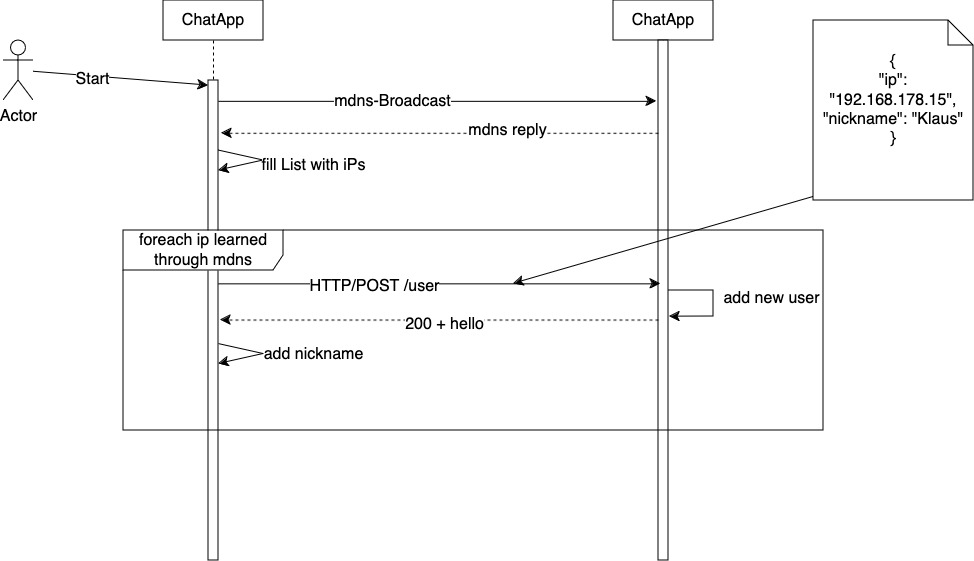
\includegraphics[scale=0.4]{Images/Initialisierung_Sequenzdiagramm.jpg}
    \captionbelow{Initialisierung}
\end{figure}
\\
\\
Nachdem man dem Chatroom beigetreten ist können Nachrichten verschickt werden. Der User schreibt eine Nachricht. 
Um diese Nachricht zu verschicken muss der Client in der Userliste alle IP Adressen der Teilnehmer nachschauen. Die Nachricht wird anschließend 
an jede einzelne IP Adresse geschickt. Das Versenden der Nachrichten findet ebenfalls mittels HTTP statt.
\begin{figure}[h]
    \centering
    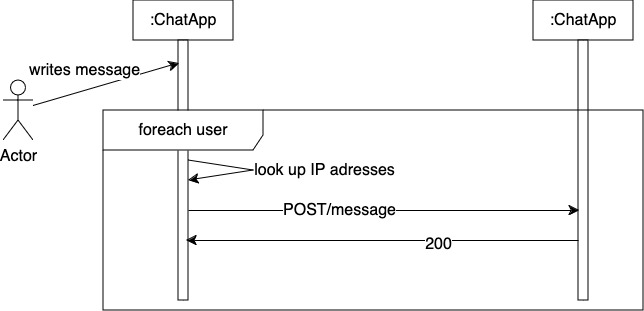
\includegraphics[scale=0.4]{Images/Conversation_Sequenzdiagramm.jpg}
    \captionbelow{Kommunikation}
\end{figure}
\\
Um den Chatroom zu verlassen wird wieder über HTTP eine Exitmessage an alle Teilnehmer gesendet. Die Exitmessage enthält wie die Startmessage den eigenen Namen und IP Adresse.
Der User wird von den anderen Teilnehmern aus der Userliste entfernt und der Client ist somit dem Chatroom ausgetreten. 
\begin{figure}[h]
    \centering
    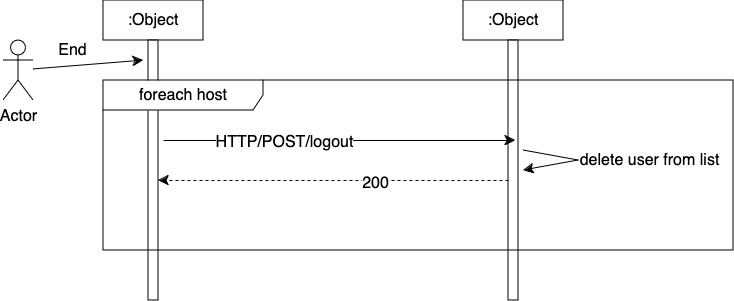
\includegraphics[scale=0.4]{Images/Exit_Sequenzdiagramm.jpg}
    \captionbelow{Exit}
\end{figure}
\\

\subsection{Aufbau und Komponenten}
Der Chat client setzt sich im wesentlichen zusammen aus:
\begin{itemize}
    \item DiscoveryService
    \item Transmitter
    \item Receiver
    \item ConfigData
    \item Message types
\end{itemize} 
Um mit dem chatten starten zu können wird der DiscoveryService benötigt. 
Er ist für den Multicast und das Eintragen der Teilnehmer in die Userliste verantwortlich,
Der Receiver ist für das Empfangen der Startmessage, der normalen Nachrichten und der Exitmessage zuständig.
Der Transmitter übernimmt die Funktion des Sendens der Nachrichten. 
In der ConfigData ist die Userliste angelegt, mit allen eingetragenen Teilnehmern des Cahtrooms und die eigenen Daten.
Die Message types definieren die einzelnen Typen und den Aufbau der unterschiedlichen Messagearten. Diese unterteilen sich in StartMessage, Message und ExitMessage.

\subsection{Funktionalität}
%Wird die Anwendung gestartet beginnt der DiscoveryService mit einem Multicast nach anderen Teilnehmern zu suchen. Hierfür wurde die zeroconf library verwendet.
%....
%Die gefundenen Teilnehmer werden mit ... in die angelegte UserLsite der ConfigData eingetrage....
%Die ConfigData besteht aus dem eigenem Namen, der eigenen IP Adresse, die mithilfe der Klasse IPv4Adress herausgesucht wird und der Portnummer.
%Des Weiteren ist in der ConfigData die Userliste angelegt. Die User sind in einem Dictonary angelegt, wobei jeder IP Adresse der passende Name zugeordnet wird.








